\subsection*{Anhang}
\label{anhang}
%TODO: Anhang Fixen
\appendix

\begin{figure}[htb]
    \centering
    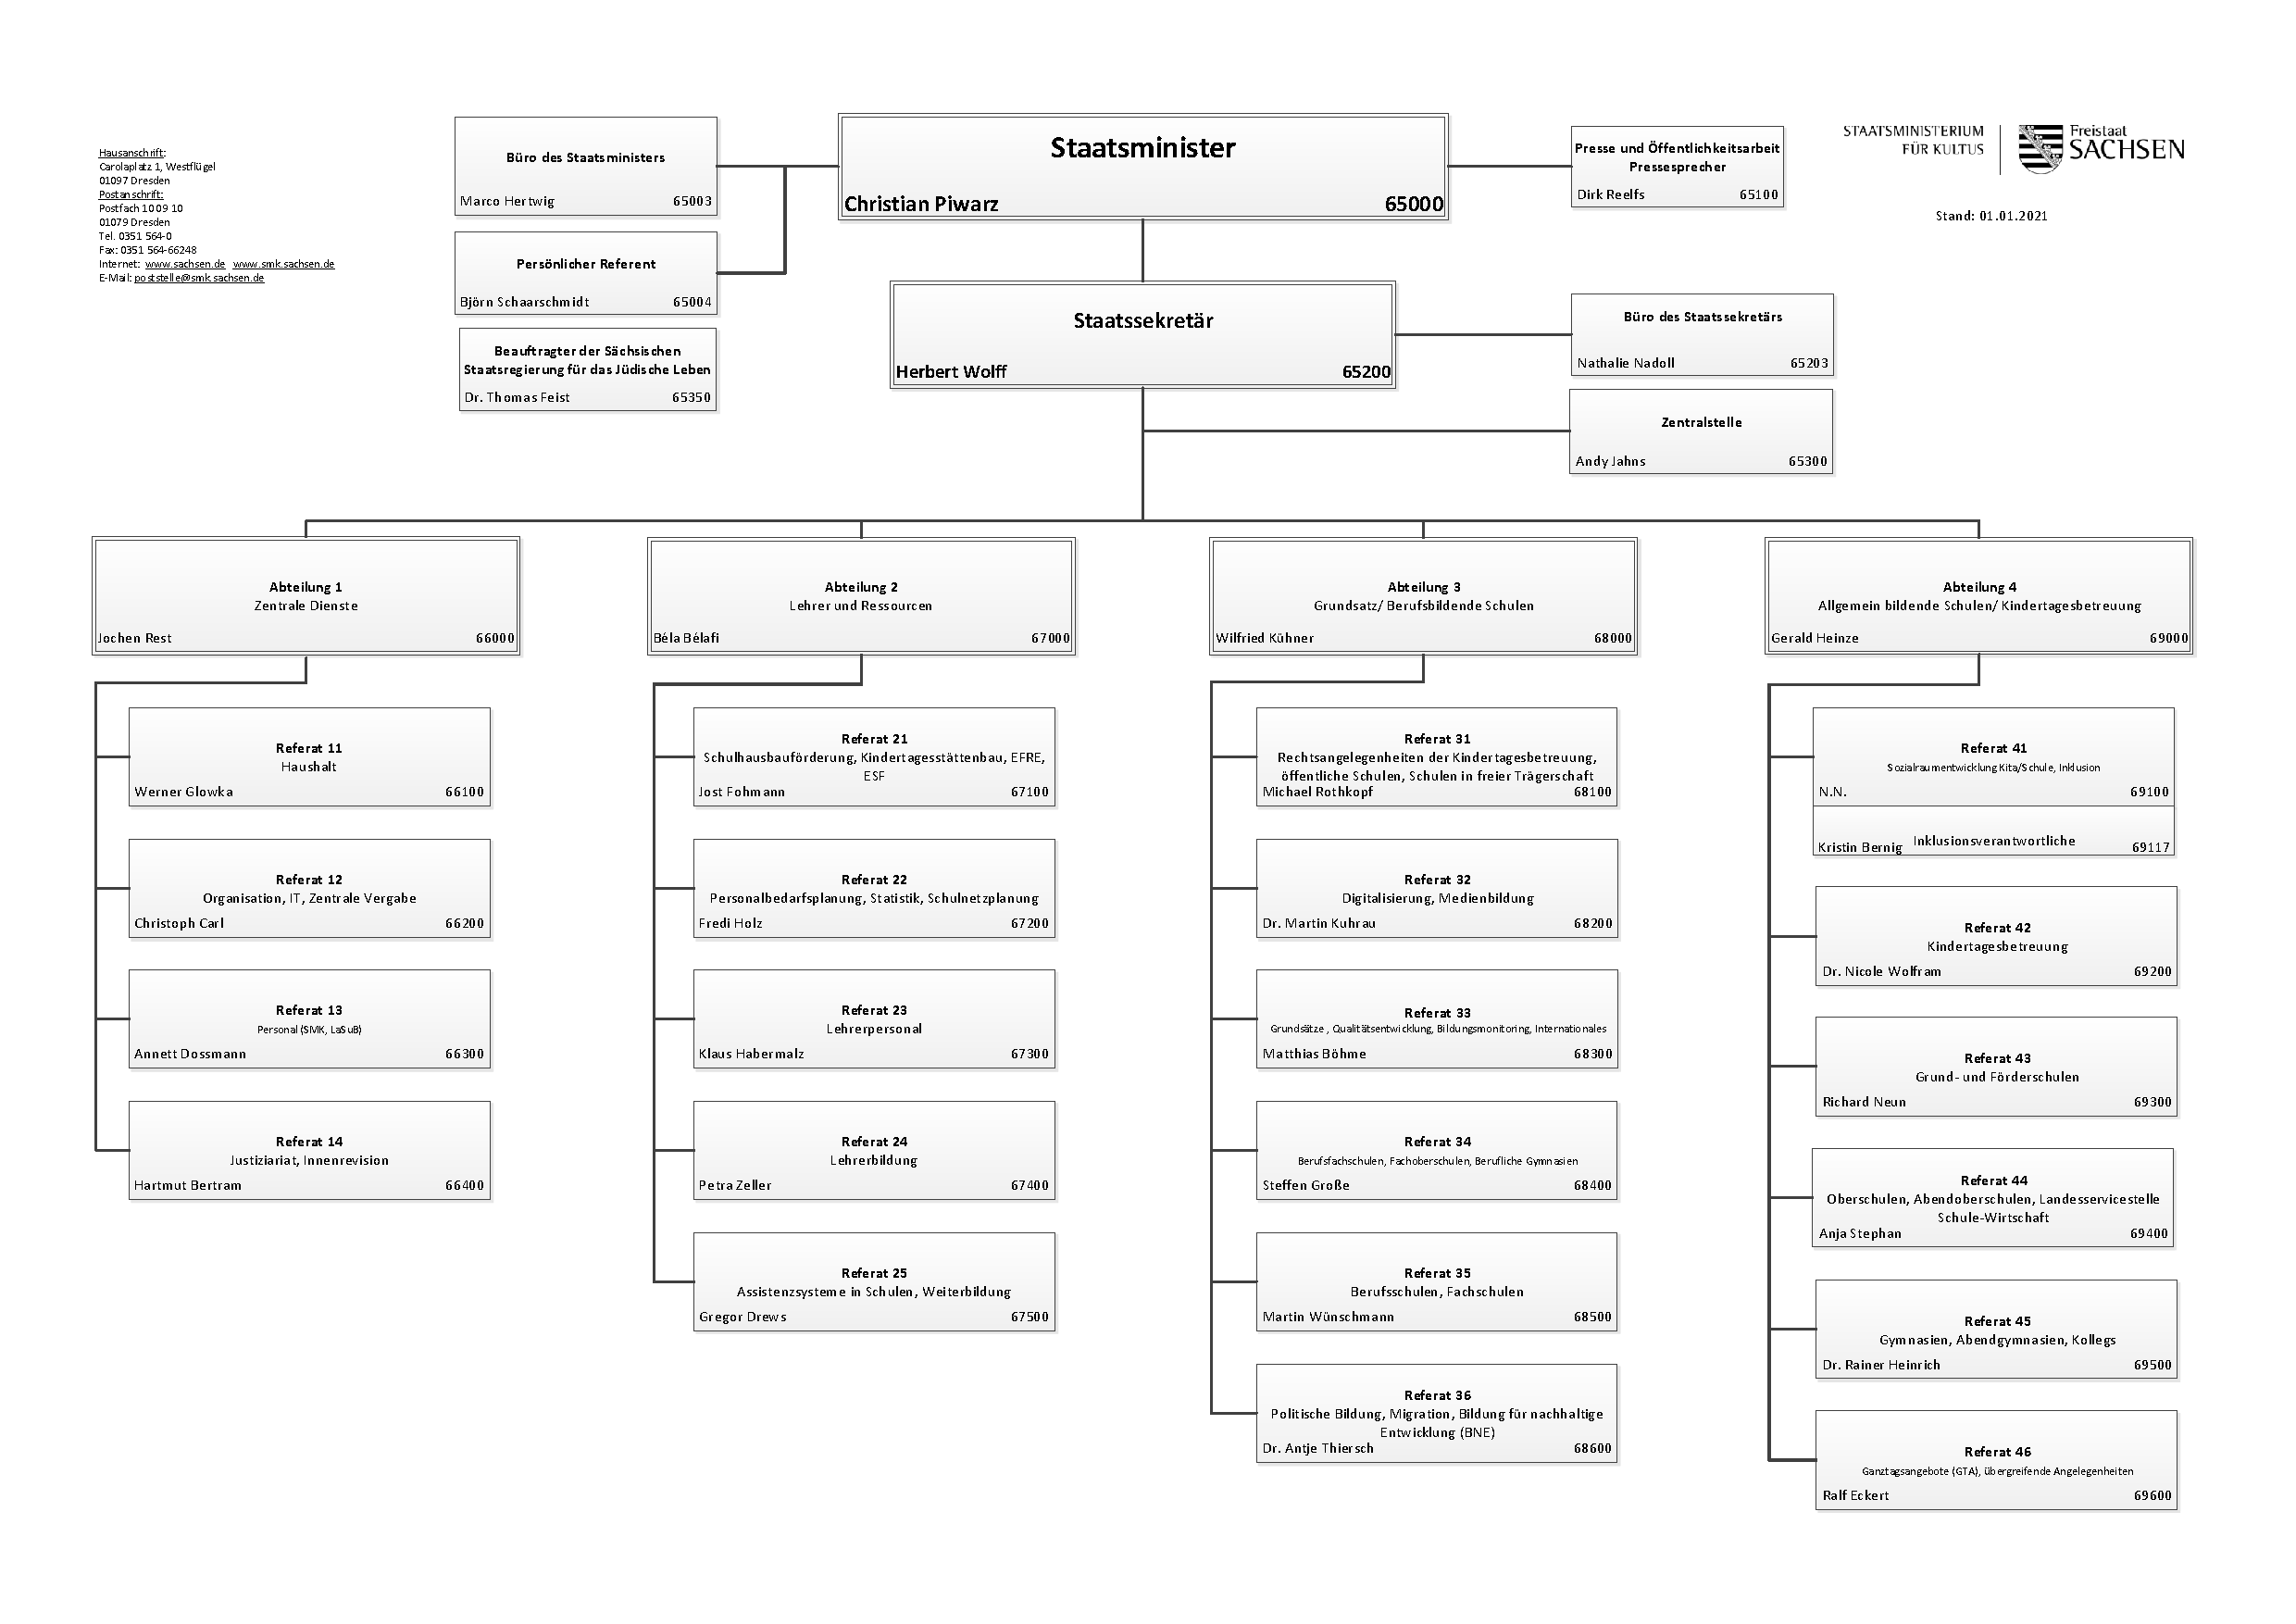
\includegraphics[angle=90, page=1,height=0.90\textheight, keepaspectratio]{anhang/abb/21_01_06_Organigramm_SMK.pdf}
    \caption[Beschreibung]{Organigramm}
    \label{abb:Organigramm}
\end{figure}

\begin{figure}[htb]
    \centering
    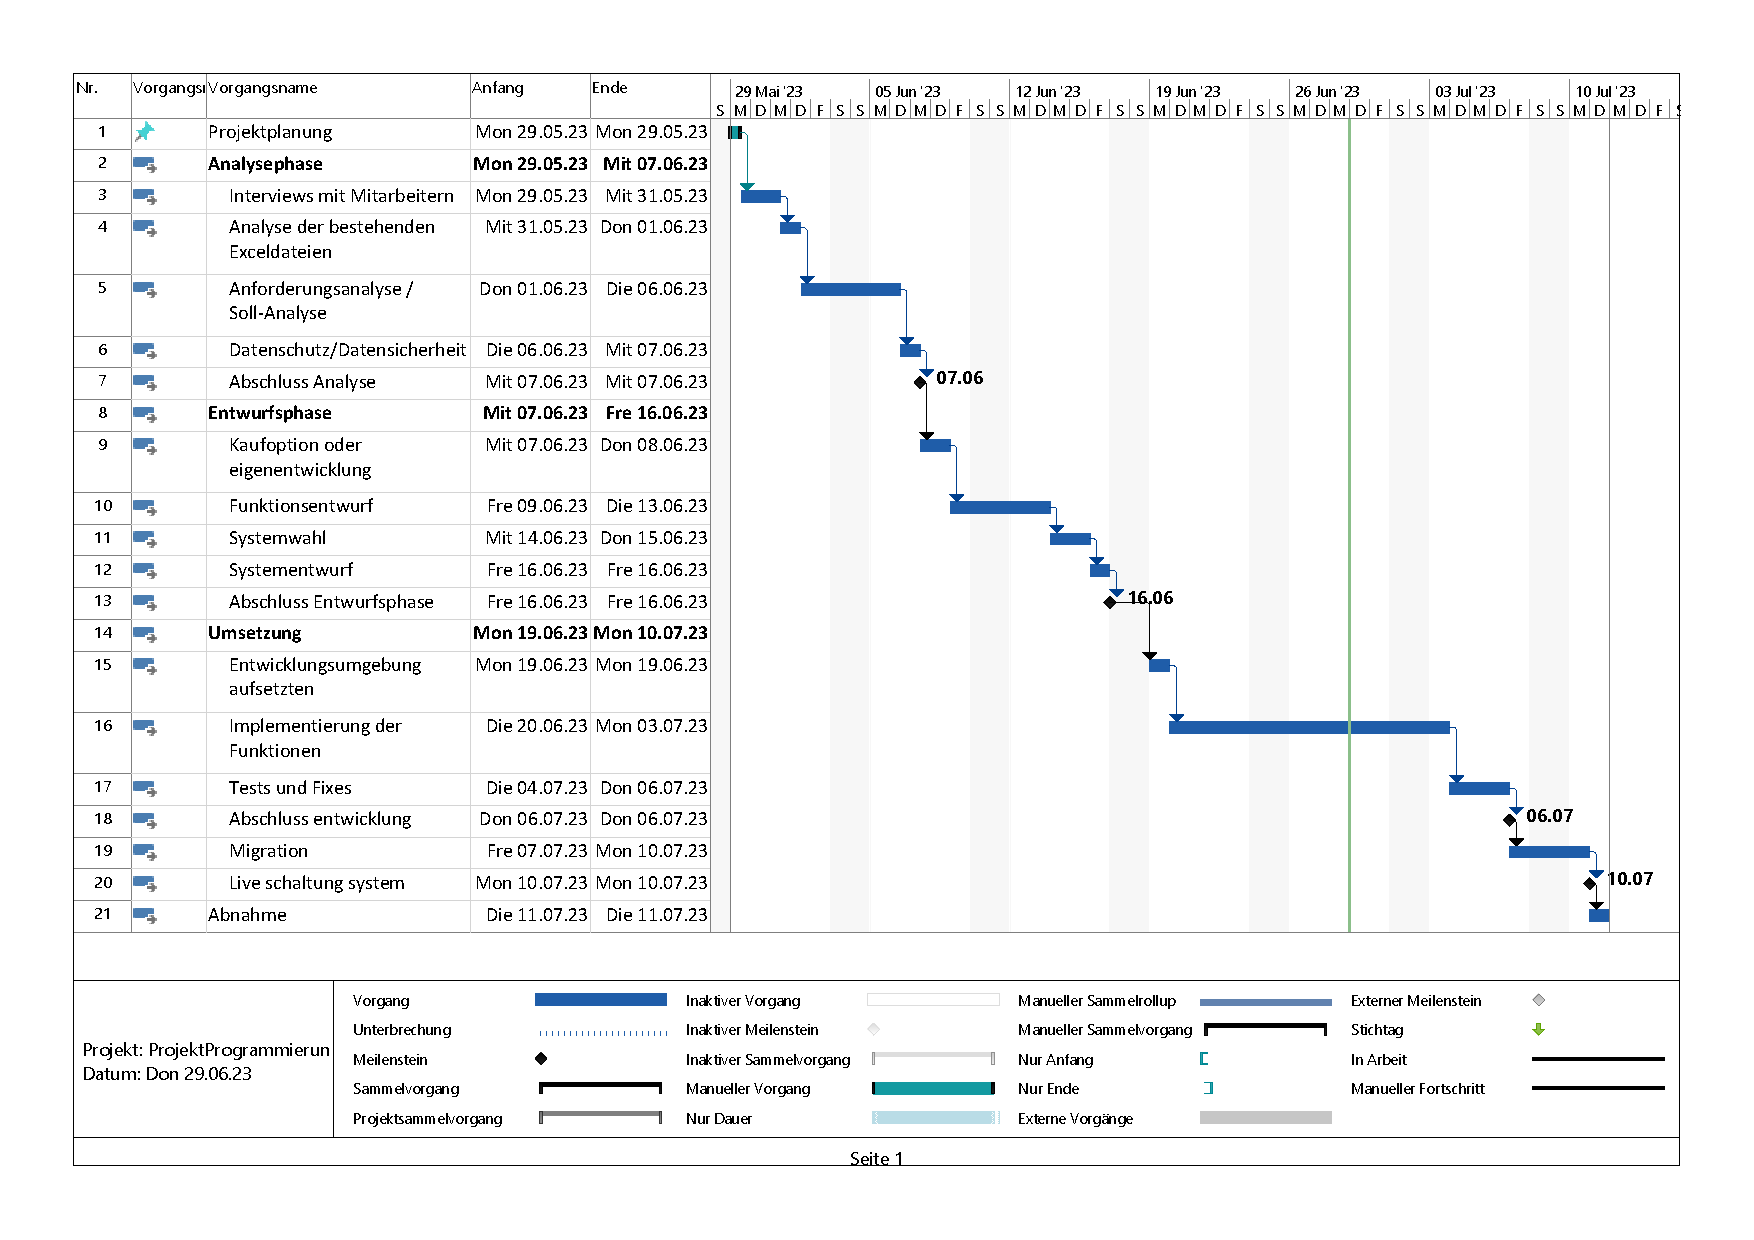
\includegraphics[angle=90, page=1,height=0.90\textheight, keepaspectratio]{anhang/abb/ProjektProgrammierungZeitplan.pdf}
    \caption[Beschreibung]{Gantt}
    \label{abb:Gantt}
\end{figure}

\begin{figure}[htb]
    \centering
    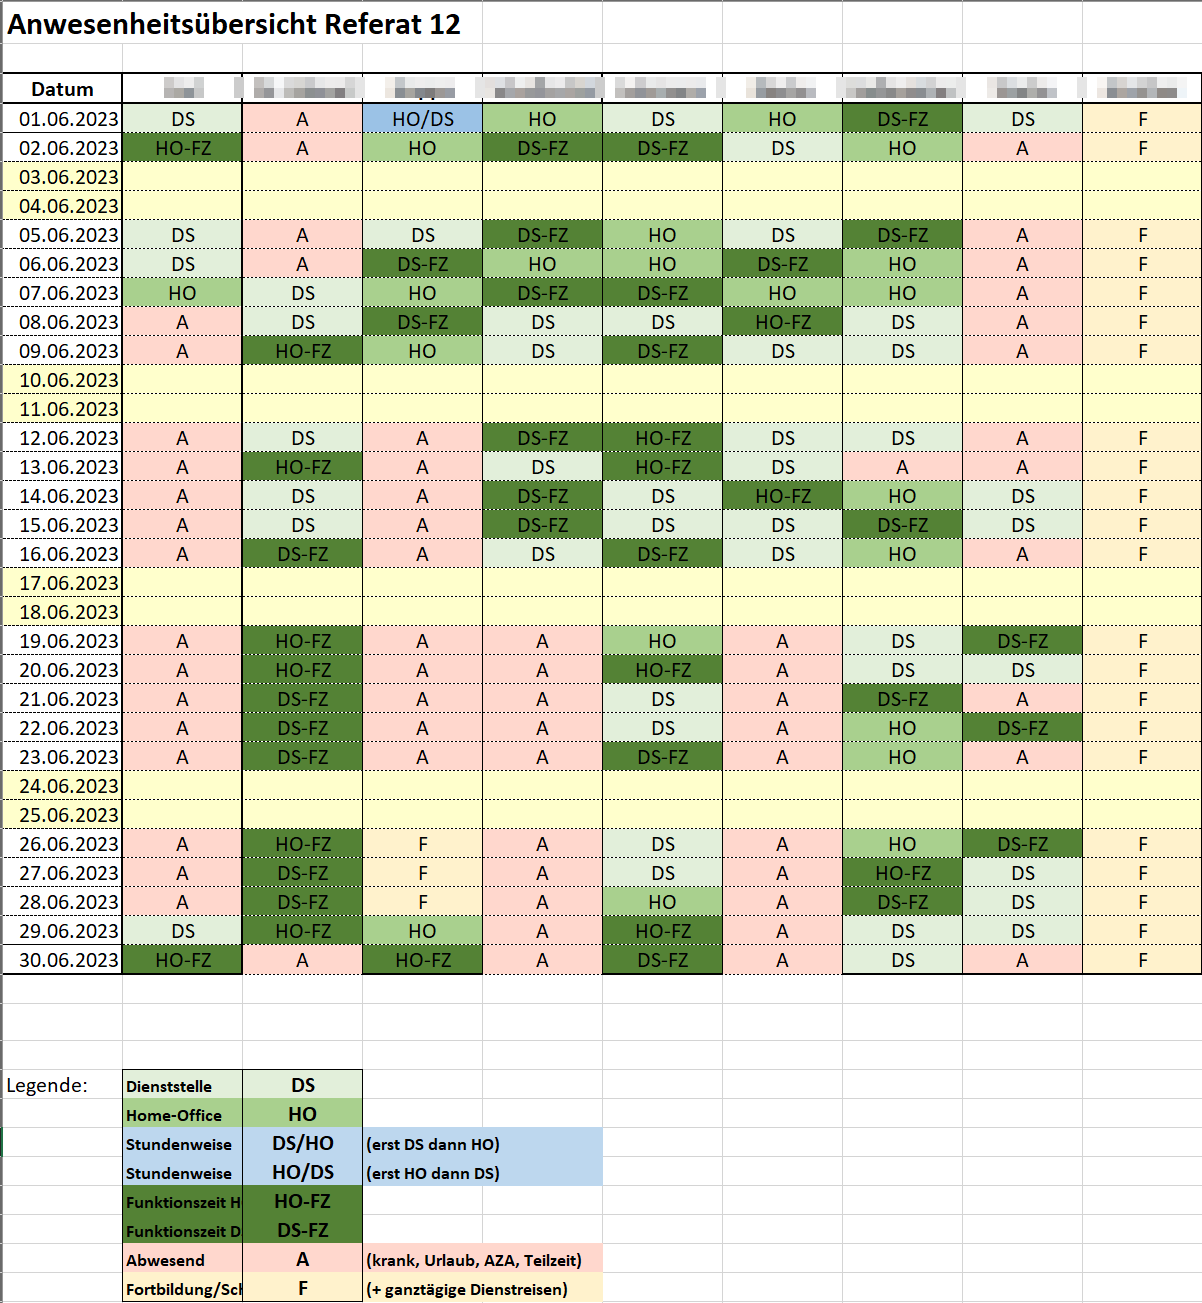
\includegraphics[page=1,height=1\textwidth]{anhang/abb/Tabelle.png}
    \caption[Beschreibung]{Referenztabelle}
    \label{abb:Ausgangstabelle}
\end{figure}


\begin{figure}[htb]
    \centering
    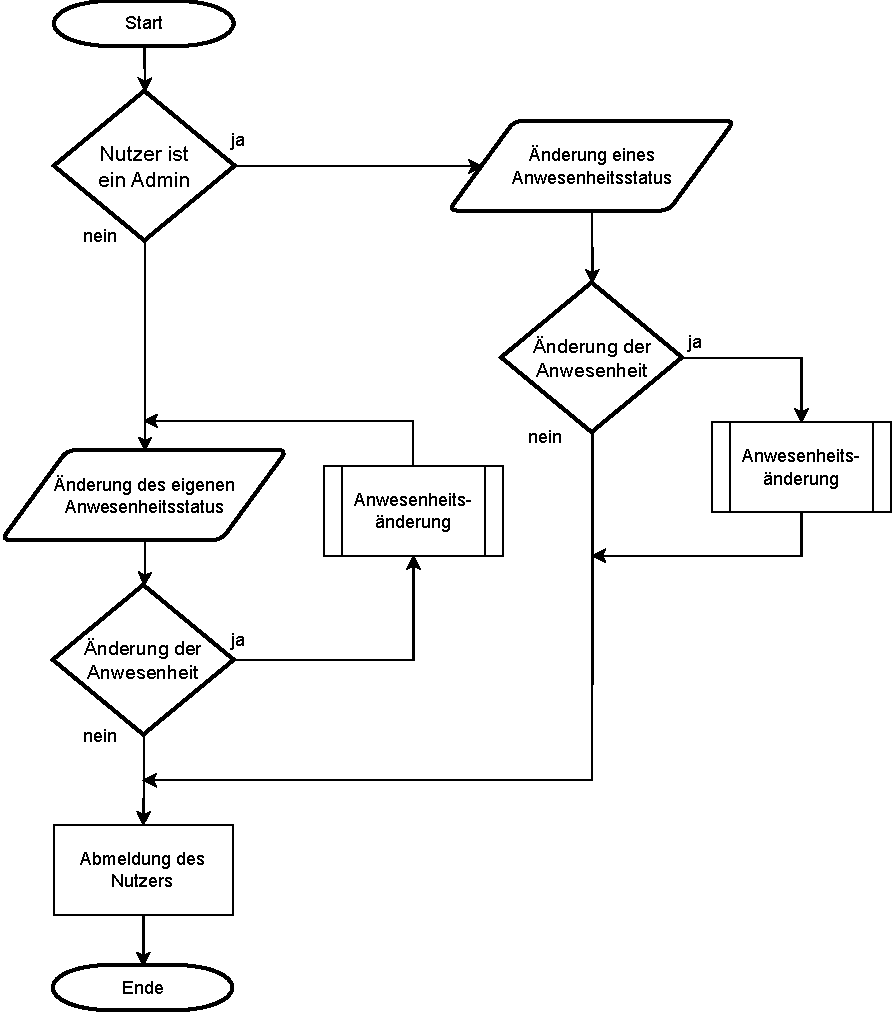
\includegraphics[width=0.9\textwidth,angle=0]{anhang/abb/PAP_Kurz.pdf}
    \caption[Beschreibung]{PAP änderungsvorgang von Anwesenheiten}
    \label{abb:PAP}
\end{figure}

\begin{figure}[htb]
    \centering
    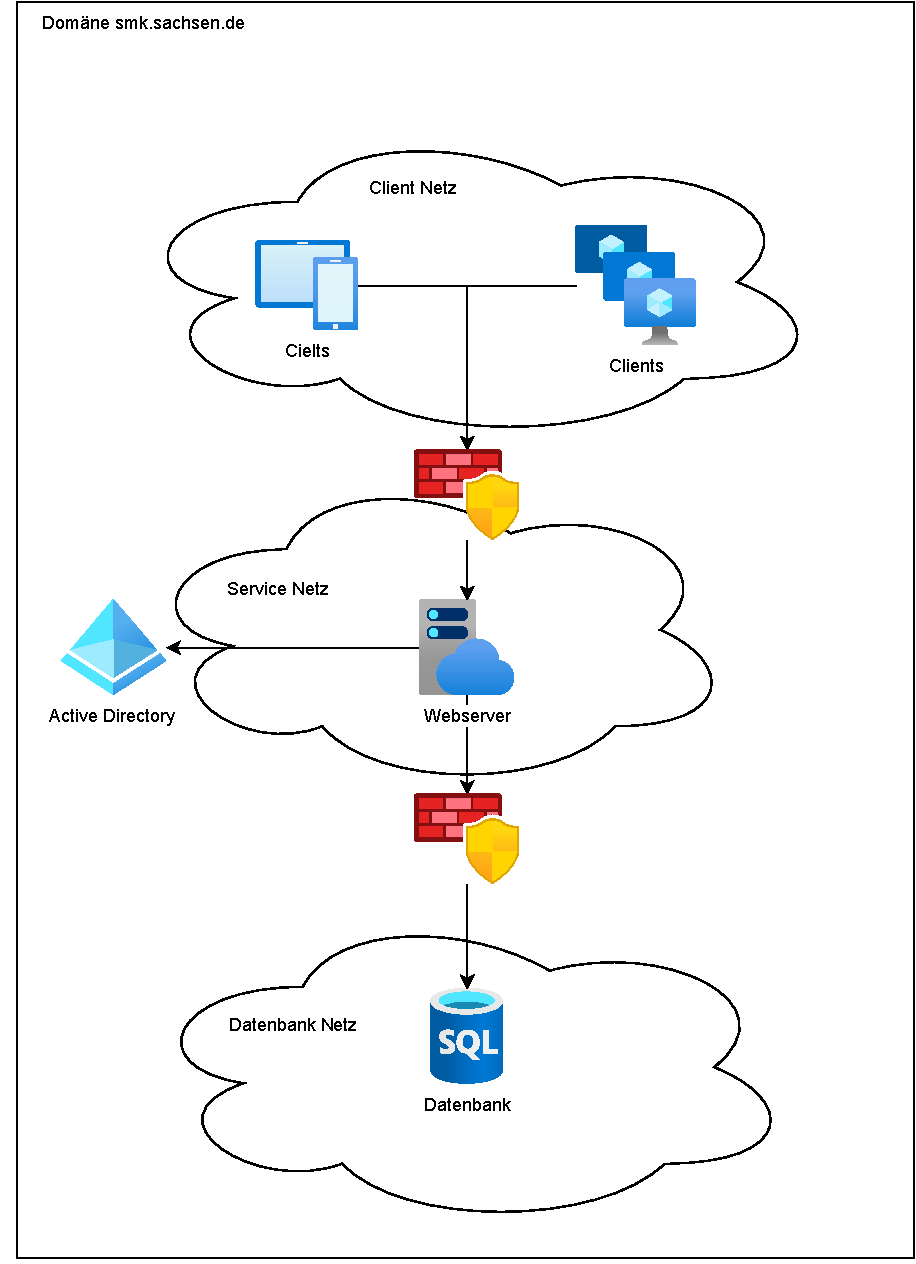
\includegraphics[width=0.9\textwidth,angle=0]{anhang/abb/Systemarchitektur.pdf}
    \caption[Beschreibung]{Systemarchitektur}
    \label{abb:Systemarchitektur}
\end{figure}

\begin{figure}[htb]
    \centering
    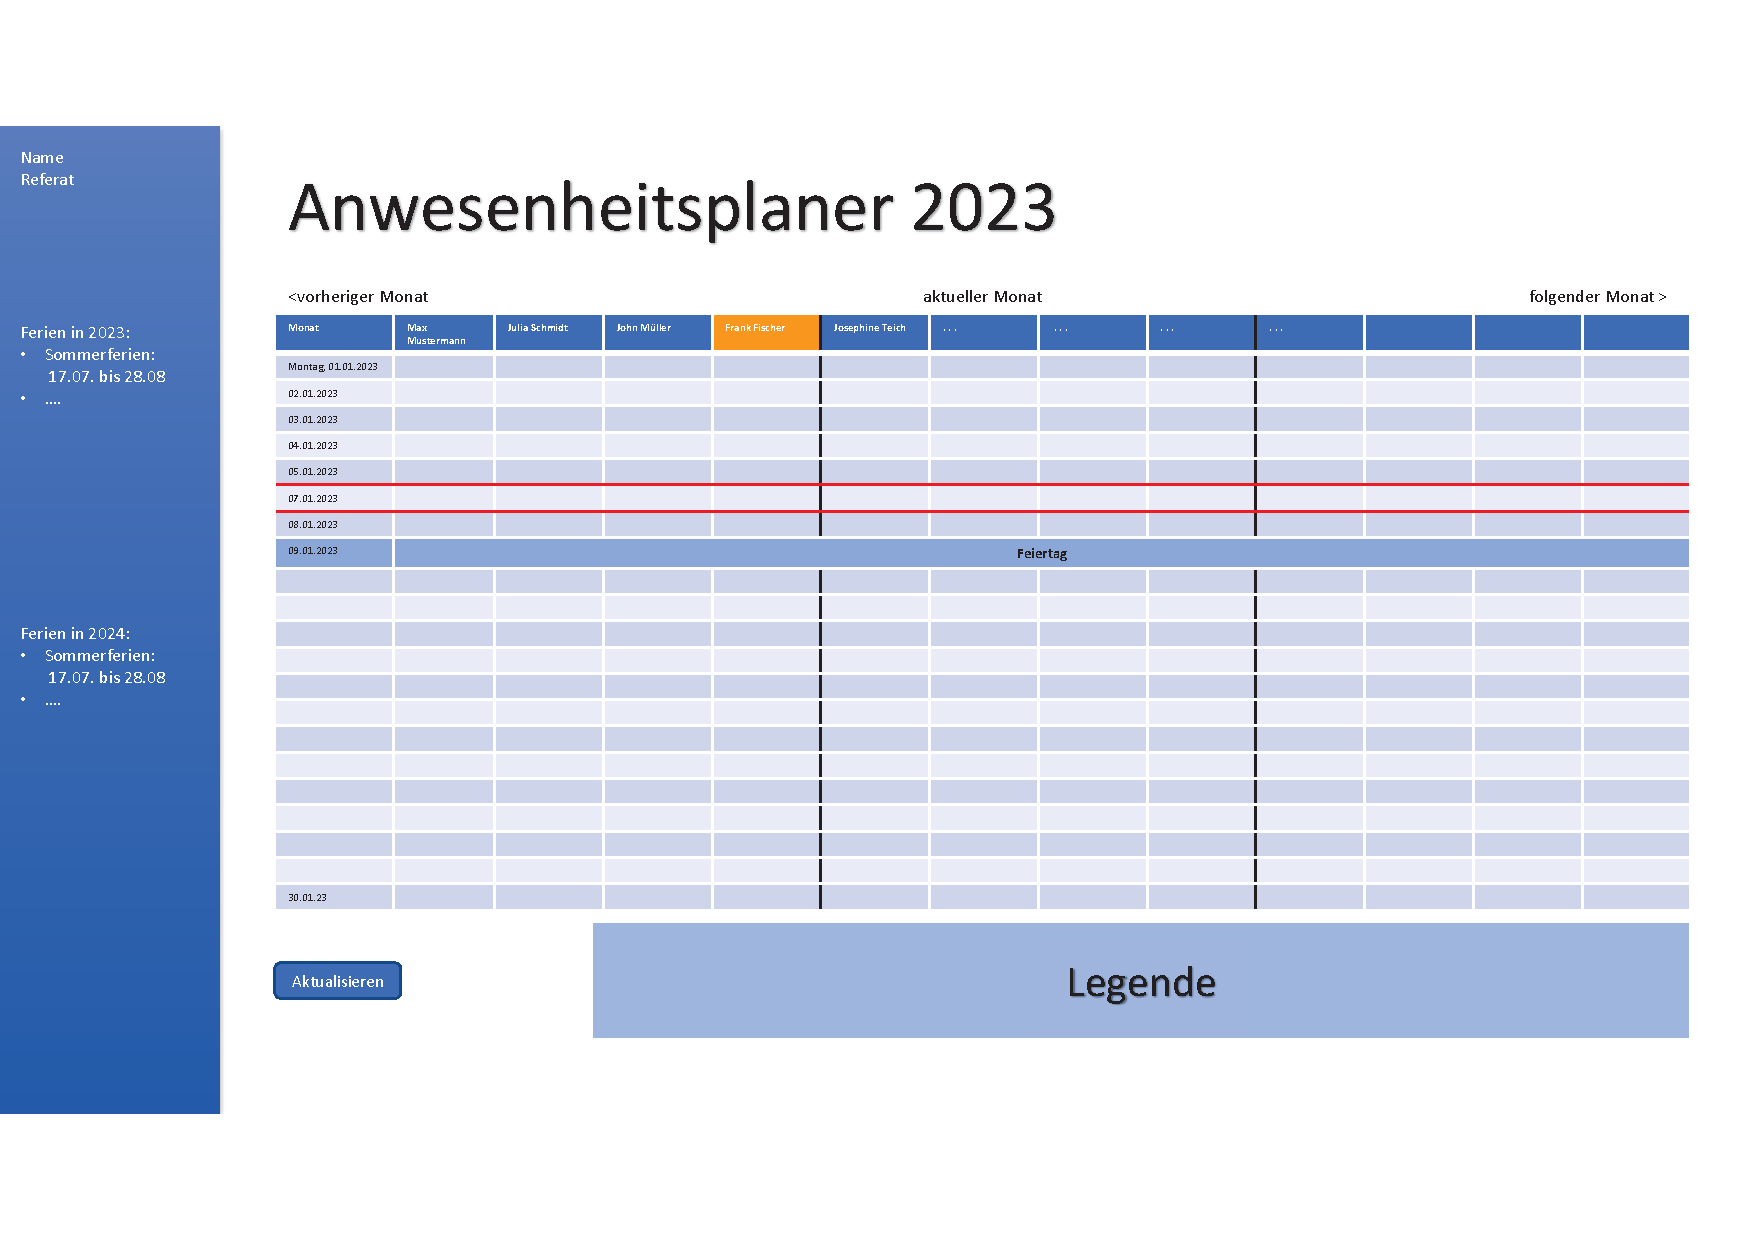
\includegraphics[angle=90, page=1,height=0.90\textheight, keepaspectratio]{anhang/abb/gui.pdf}
    \caption[Beschreibung]{GUI Entwurf}
    \label{abb:GUIEntwurf}
\end{figure}

\begin{figure}[htb]
    \centering
    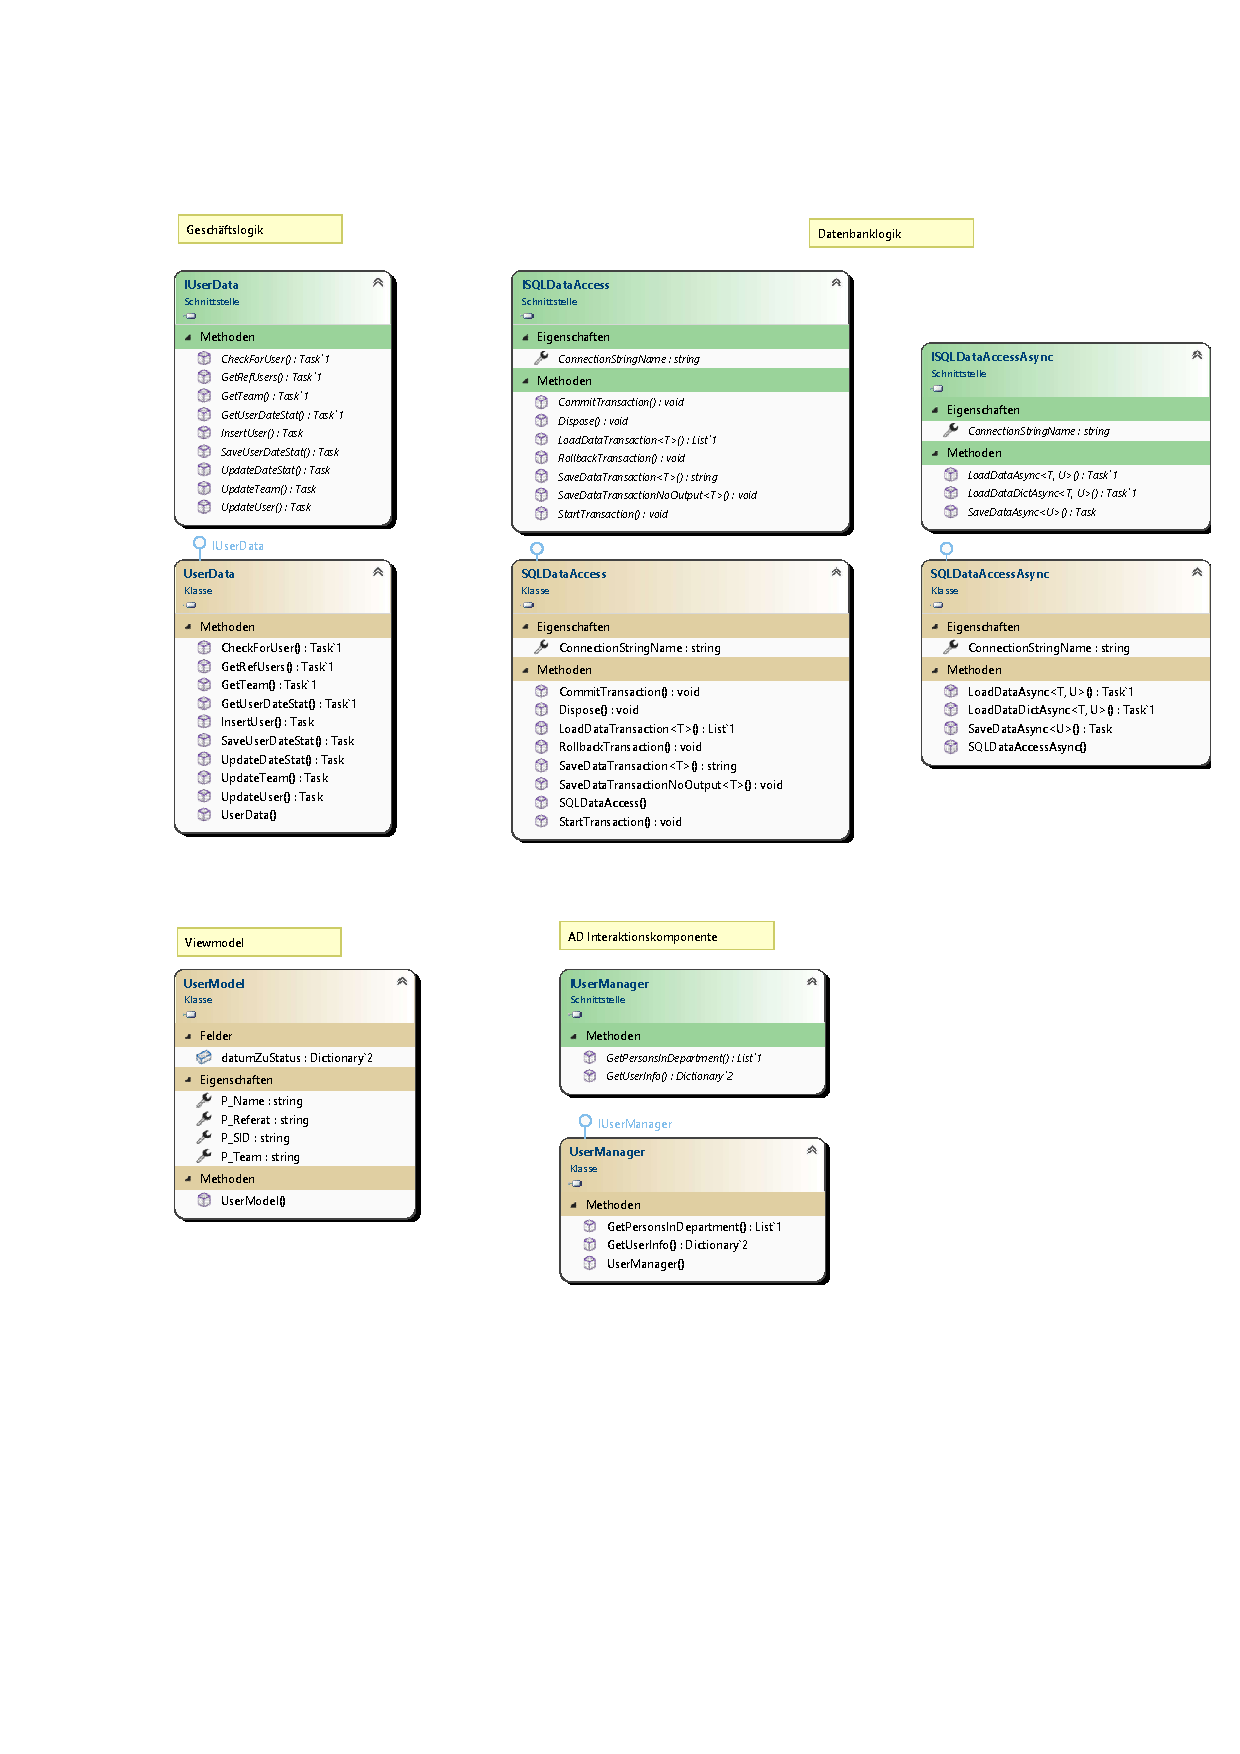
\includegraphics[width=1\textwidth,angle=0]{anhang/abb/Klassendiagramm.pdf}
    \caption[Beschreibung]{Klassendiagramm}
    \label{abb:Klassendiagramm}
\end{figure}